
\subsection{Robustness Improvement through EPA}

\paragraph{EPA improves robustness. }The results in Table~\ref{tab:main} shows the effectiveness of EPA in  robustness to ASR errors. Remarkably, EPA outperformed existing text-based and audio-based augmentation, showing substantial improvement in JGA and named entity accuracy. It also surpassed the previous best-performing model, Olisia, particularly  in challenging environments.

\paragraph{Effectiveness of keyword-specific error.} In Table~\ref{tab:main}, we present an ablation study to evaluate the effectiveness of keyword-level augmentation. We found that adding keyword-specific ASR errors improved DST performance across all environments and was particularly helpful in enhancing the robustness of named entity accuracy. Additional experiments, including generalization to other backbones and tasks, as well as statistical significance analysis, are provided in Appendix~\ref{app:exp_main}.


\subsection{Comparison with Error Correction Models}
\begin{table}[t]
\centering
\resizebox{\columnwidth}{!}{%
\begin{tabular}{l|cc|cc|cc}
\hline
\multicolumn{1}{c|}{\multirow{2}{*}{Method}} &
  \multicolumn{2}{c|}{Weak-ASR} &
  \multicolumn{2}{c|}{Noised-ASR} &
  \multicolumn{2}{c|}{Strong-ASR} \\\cline{2-7} 
\multicolumn{1}{c|}{} & JGA & N-acc & JGA & N-acc & JGA & N-acc \\ \hline
Baseline & 29.88 & 45.76 & 29.70 & 46.77 & 34.87 & 52.07 \\ 
+ \textsc{Correction model 1} & 23.30 & 41.50 & 23.96 & 42.86 & 26.68 & 46.14 \\ 
+ \textsc{Correction model 2} & 30.14 & 46.79 & 29.82 & 47.68 & 34.62 & 52.00 \\ 
+ EPA (with GPT, ours) & \textbf{32.39} & \textbf{51.12} & \textbf{32.24} & \textbf{52.70} & \textbf{36.61} & \textbf{55.87} \\ \hline
\end{tabular}%
}
\caption{Comparison with ASR error correction models under different ASR conditions. }
\label{tab:err_correction}
\end{table}

In Table~\ref{tab:err_correction}, we compare our method with two ASR error correction approaches. For \textsc{Error Correction Model 1}, We fine-tuned a pre-trained on 300 hours of ASR-errored and gold transcription pairs (same as in Section~\ref{sec:method_step1}) in a seq2seq manner, minimizing \( L = - \sum_{i=1}^{N} \log P(g_i \mid e_i) \),
where \(g_i\) and \(e_i\) denote the gold and errored transcriptions, respectively. 
Training used early stopping (patience=3) with batch size 16.
For \textsc{Error Correction Model 2}, we adopted an off-the-shelf\footnote{url{https://huggingface.co/oliverguhr/spelling-correction-english-base}} text correction model to revise typos and transcription errors. Each model corrected the test transcriptions from the weak, noised, and strong ASR systems before DST evaluation. 
As in the table, \textsc{Correction model 1} underperforms the baseline, often altering named entities unnecessarily (e.g., "Grifon" $\rightarrow$ "Bristol"), likely due to limited training diversity. 
\textsc{Correction model 2} yields minor improvements, while our EPA achieves the highest robustness across all ASR conditions.



\subsection{Qualitative Assessment of EPA Method}
\label{sec:quality}

\begin{table}[!ht]
\centering
\resizebox{0.9\columnwidth}{!}{%
\begin{tabular}{l|rrr}
\hline
Method & \multicolumn{1}{r|}{\makecell{Uniq. \\ Words}} & \multicolumn{1}{r}{\makecell{NE.chg \\ \text{[ \% ]}}}  & \multicolumn{1}{r}{\makecell{Pronoun  \\ Sim.\text{[\%]}}}  \\ \hline
Baseline         & 1                          & -    & -  \\\hline
AEDA \cite{aeda} & \multicolumn{1}{l}{1.00$\times$} & 44.29   & 91.57         \\
EDA \cite{eda}   & \multicolumn{1}{l}{0.86$\times$} & 70.03   & 61.14         \\
BT \cite{BT}     & \multicolumn{1}{l}{1.21$\times$} & 73.46   & 77.17         \\
TTS-ASR       & \multicolumn{1}{l}{1.01$\times$} & 38.84 & \textbf{98.93}  \\
Translating           & \multicolumn{1}{l}{0.84$\times$} & 39.59 & 94.07           \\
\rowcolor[gray]{0.9}  EPA     & \multicolumn{1}{l}{\textbf{1.81}$\times$} & \textbf{95.47} & 91.57  \\
\quad w/o Keyword Err. & \multicolumn{1}{l}{1.57$\times$} & 68.81  & 93.14      \\ 
\hline
\end{tabular}%
}
\caption{Assessment of EPA dataset quality: Unique word increased rate, Named entity changed rate (NE.chg), and pronunciation similarity. }
\label{tab:quality}
\end{table}

% Error analysis of EPA especially on keyword.
% Assessment of EPA dataset quality across three key aspects (Uniq.Words, NE.differ, AudioSim.) 

\paragraph{Automatic evaluation.} Although Table~\ref{tab:main} confirms EPA's effectiveness, it remains unclear whether the LLM-generated augmentations truly reflect diverse, keyword-focused ASR-style errors. To this end, we perform the quality analysis based on three metrics (Table~\ref{tab:quality}): the unique word increase rate, named entity change rate, and pronunciation similarity with original sentence. The results show that EPA achieves remarkable diversity in unique words (1.81×) and the highest named entity change rate (95.47\%), while maintaining high pronunciation similarity (91.57\%). Notably, keyword-level augmentation plays a key role in enhancing named entity variability, increasing the change rate from 68.81\% to 95.47\%.


\paragraph{Comparison with Authentic ASR Errors.}
\label{app:appendix-edit}
\begin{figure}[h]
  \centering
  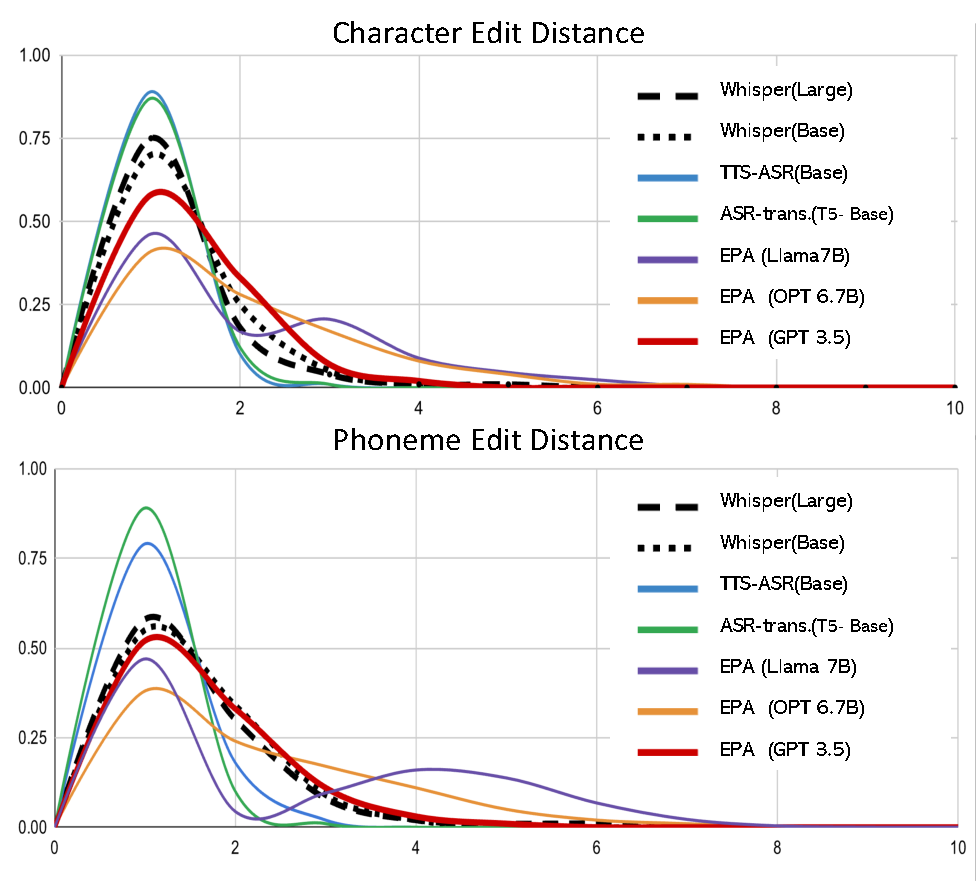
\includegraphics[width=.95\columnwidth]{img/edit_2025.pdf}
   \caption{Distribution of edit distance. The x-axis represents edit distances, and the y-axis represents the corresponding ratio.}
   \label{fig:edit}
\end{figure}

\begin{table}[t]
\centering
\resizebox{.9\columnwidth}{!}{%
\begin{tabular}{l|rr|rr}
\toprule
\multirow{2}{*}{Method} & \multicolumn{2}{c|}{Text Dist.($\downarrow$)}                     & \multicolumn{2}{c}{Phoneme Dist.($\downarrow$)}                  \\\cline{2-5}
                        & \multicolumn{1}{c}{ASR-L} & \multicolumn{1}{c|}{ASR-B} & \multicolumn{1}{c}{ASR-L} & \multicolumn{1}{c}{ASR-B} \\\hline
TTS-ASR \small{(Whisper-B)}  & 0.030  & 0.048 & 0.056          & 0.061        \\
TTS-ASR \small{(Whisper-S)} & 0.030  & 0.048 & 0.070           & 0.077          \\
ASR trans. \small{(T5-base)}            & \textbf{0.025} & 0.039 & 0.104          & 0.116          \\ \hline
EPA \small{(Llama2 7B)}    & 0.218 & 0.123 & 0.204          & 0.256          \\
EPA \small{(OPT 6.7B)}      & 0.115 & 0.106 &  0.071  &  0.091    \\
EPA \small{(GPT 3.5)}      & 0.033 & \textbf{0.010}  & \textbf{0.009} & \textbf{0.007} \\ 

\toprule
\end{tabular}%
}
\caption{Distribution distance (JSD) between Whisper Large/Base model and simulation dataset. (ASR‑L=Whisper Large, ASR‑B=Whisper Base). }
\label{tab:edit}
\end{table}

In this analysis, we explored the similarity between simulated ASR errors and authentic ASR errors from the perspective of edit distance. Specifically, we examined the distribution of edit distances in simulated data and in errors produced by Whisper large/base models, considering both character- and phoneme-level representations (Figure~\ref{fig:edit}). To quantify the distributional differences, we computed the Jensen-Shannon Divergence (JSD), a symmetric variant of the Kullback-Leibler divergence (Table~\ref{tab:edit}).

Our experiments yielded several noteworthy findings.
Notably, the LLM-simulated errors closely matched the distribution of real ASR errors, particularly at the phoneme level.
This suggests that LLMs can effectively capture pronunciation-level variations and generate realistic ASR-style distortions.
In contrast, errors produced by TTS-based synthesis or ASR-translation models exhibited larger divergence from real ASR patterns, likely due to their tendency to generate more diverse but less phonetically grounded outputs.



\paragraph{Human evaluation.} To further verify the quality of our EPA method, we conducted a human evaluation using 100 sentence pairs, each consisting of an original sentence and its augmented counterpart, with two human evaluators. Participants rated how likely the change resembled an ASR error on a 4-point Likert scale, where 1 indicated "not like an ASR error" and 4 indicated "clearly an ASR error." The average rating was 3.22 with moderate inter-rater agreement   (Gwet’s AC2 \cite{gwet} = 0.590), suggesting that most EPA-generated edits were perceived as realistic ASR errors. Details on the evaluation metric and human evaluation are provided in Appendix~\ref{app:quality}.


\subsection{Error Analysis}


We additionally analyze the impact of keyword augmentation by examining how it influences specific error types in DST predictions. Table~\ref{tab:err} presents the percentage reduction in error rates compared to the baseline. The results demonstrate that EPA is effective in "Wrong" and "Ignore" error types, and keyword augmentation highly contributed to this improvement by decreasing the error rate from 5.29\% to 8.19\%. Interestingly, while keyword augmentation led to substantial reductions in "Wrong" errors, it also caused a slight increase in "Spurious" errors. This may be because the model, after repeatedly seeing phonetic noise around slot values, becomes overly sensitive and starts hallucinating unmentioned slots. A potential mitigation is to introduce an additional loss term for slot presence prediction \cite{trippy,kim2019efficient} , helping the model better distinguish between mentioned and unmentioned slots.

% error type
\begin{table}[t]
\centering
\resizebox{0.95\columnwidth}{!}{%
\footnotesize{
\begin{tabular}{lccc}
\hline
\multicolumn{1}{l|}{\multirow{2}{*}{Method}} &
  \multicolumn{3}{c}{Error Type} \\ \cline{2-4} 
\multicolumn{1}{l|}{} &
  \multicolumn{1}{l|}{Wrong} &
  \multicolumn{1}{l|}{Ignore} &
  \multicolumn{1}{l}{Spurious} \\ \hline

  \multicolumn{4}{c}{Noised Audio} \\ \hline
\multicolumn{1}{l|}{Baseline} &
  \multicolumn{1}{c|}{\begin{tabular}[c]{@{}c@{}}{\color{blue}$\triangledown$}0\%\\ \scriptsize{(6237)}\end{tabular}} &
  \multicolumn{1}{c|}{\begin{tabular}[c]{@{}c@{}}{\color{blue}$\triangledown$}0\%\\ \scriptsize{(3654)}\end{tabular}} &
  \begin{tabular}[c]{@{}c@{}}{\color{blue}$\triangledown$}0\%\\ \scriptsize{(2027)}\end{tabular} \\ \hline
\multicolumn{1}{l|}{EPA w/o Key-aug} &
  \multicolumn{1}{c|}{\begin{tabular}[c]{@{}c@{}}{\color{blue}$\triangledown$}5.29\%\\ \scriptsize{(5907)}\end{tabular}} &
  \multicolumn{1}{c|}{\begin{tabular}[c]{@{}c@{}}{\color{blue}$\triangledown$}3.72\%\\ \scriptsize{(3518)}\end{tabular}} &
  \begin{tabular}[c]{@{}c@{}}{\color{blue}$\triangledown$}\textbf{6.31}\%\\ \scriptsize{(1899)}\end{tabular} \\ \hline
\multicolumn{1}{l|}{EPA} &
  \multicolumn{1}{c|}{\begin{tabular}[c]{@{}c@{}}{\color{blue}$\triangledown$}\textbf{8.19}\%\\ \scriptsize{(5726)}\end{tabular}} &
  \multicolumn{1}{c|}{\begin{tabular}[c]{@{}c@{}}{\color{blue}$\triangledown$}\textbf{7.25}\%\\ \scriptsize{(3389)}\end{tabular}} &
  \begin{tabular}[c]{@{}c@{}}{\color{blue}$\triangledown$}1.33\%\\ \scriptsize{(2000)}\end{tabular} \\ \hline



  
% \multicolumn{4}{c}{High-acc ASR (WER<0.03)} \\ \hline
% \multicolumn{1}{l|}{Baseline} &
%   \multicolumn{1}{c|}{\begin{tabular}[c]{@{}c@{}}
%   {\color{blue}$\triangledown$}0\%\\ \scriptsize{(4844)}\end{tabular}} &
%   \multicolumn{1}{c|}{\begin{tabular}[c]{@{}c@{}}{\color{blue}$\triangledown$}0\%\\ \scriptsize{(3493)}\end{tabular}} &
%   \begin{tabular}[c]{@{}c@{}}{\color{blue}$\triangledown$}0\%\\ \scriptsize{(1862)}\end{tabular} \\ \hline
% \multicolumn{1}{l|}{EPA w/o Key-aug} &
%   \multicolumn{1}{c|}{\begin{tabular}[c]{@{}c@{}}{\color{blue}$\triangledown$}1.57\%\\ \scriptsize{(4769)}\end{tabular}} &
%   \multicolumn{1}{c|}{\begin{tabular}[c]{@{}c@{}}{\color{blue}$\triangledown$}\textbf{3.34}\%\\ \scriptsize{(3380)}\end{tabular}} &
%   \begin{tabular}[c]{@{}c@{}}{\color{blue}$\triangledown$}\textbf{6.52}\%\\ \scriptsize{(1748)}\end{tabular} \\ \hline
% \multicolumn{1}{l|}{EPA} &
%   \multicolumn{1}{c|}{\begin{tabular}[c]{@{}c@{}}{\color{blue}$\triangledown$}\textbf{7.16}\%\\ \scriptsize{(4497)}\end{tabular}} &
%   \multicolumn{1}{c|}{\begin{tabular}[c]{@{}c@{}}{\color{blue}$\triangledown$}2.43\%\\ \scriptsize{(3408)}\end{tabular}} &
%   \begin{tabular}[c]{@{}c@{}}{\color{blue}$\triangledown$}0.75\%\\ \scriptsize{(1848)}\end{tabular} \\ \hline

% \multicolumn{4}{c}{High-acc ASR (WER\textless0.2)} \\ \hline
% \multicolumn{1}{l|}{baseline} &
%   \multicolumn{1}{c|}{\begin{tabular}[c]{@{}c@{}}{\color{blue}$\triangledown$}0\%\\ \scriptsize{(4844)}\end{tabular}} &
%   \multicolumn{1}{c|}{\begin{tabular}[c]{@{}c@{}}{\color{blue}$\triangledown$}0\%\\ \scriptsize{(3493)}\end{tabular}} &
%   \begin{tabular}[c]{@{}c@{}}{\color{blue}$\triangledown$}0\%\\ \scriptsize{(1862)}\end{tabular} \\ \hline
% \multicolumn{1}{l|}{EPA w/o Keyword} &
%   \multicolumn{1}{c|}{\begin{tabular}[c]{@{}c@{}}{\color{blue}$\triangledown$}1.55\%\\ \scriptsize{(4769)}\end{tabular}} &
%   \multicolumn{1}{c|}{\begin{tabular}[c]{@{}c@{}}{\color{blue}$\triangledown$}3.24\%\\ \scriptsize{(3380)}\end{tabular}} &
%   \begin{tabular}[c]{@{}c@{}}{\color{blue}$\triangledown$}6.12\%\\ \scriptsize{(1748)}\end{tabular} \\ \hline
% \multicolumn{1}{l|}{EPA} &
%   \multicolumn{1}{c|}{\begin{tabular}[c]{@{}c@{}}{\color{blue}$\triangledown$}7.16\%\\ \scriptsize{(4497)}\end{tabular}} &
%   \multicolumn{1}{c|}{\begin{tabular}[c]{@{}c@{}}{\color{blue}$\triangledown$}2.43\%\\ \scriptsize{(3408)}\end{tabular}} &
%   \begin{tabular}[c]{@{}c@{}}{\color{blue}$\triangledown$}0.75\%\\ \scriptsize{(1848)}\end{tabular} \\ \hline
\end{tabular}
}
}
\caption{Ablation study with error analysis. \textbf{Wrong} indicates the model predicts incorrect values, \textbf{Ignore} refers to ignored mentioned slots, and \textbf{Spurious} denotes predicting values for unmentioned slots.  Actual error numbers are in parentheses.}
\label{tab:err}
\vspace{-14pt}
\end{table}



%  The analysis was conducted under the noised audio condition.



